\section{The Application}

The application consists of a number of indipendent nodes that comprise a graph. Each node sends and receives information to and from other nodes of the graph using \textit{Topics}.
The communication between nodes strongly relies on a publish/subscribe mechanism useful to  exchange data in a distributed system. 


\subsection{Use cases}

\textbf{Initialization}
The application is launched by executing the init.launch file. The Roslaunch tool allows to launch multiple ROS nodes as well as set several parameters for the simulation environment. the initialization process brings up the master node, roscore, the coordinator, the semanticMapInterface and Gazebo.\\
\\
Once initialized, the SemanticMapInterface loads from a specified absolute path the Terminology Box and the Assertions Box as Ontology Models.

\begin{lstlisting}[language=Java]
/**
 * Importing Tbox
 */
 tbox = ModelFactory.createOntologyModel( OntModelSpec.OWL_MEM );
 OntDocumentManager dm_tbox = tbox.getDocumentManager();
 dm_tbox.addAltEntry(SOURCE+TBOX_FILE,"file:"+TBOX_FILE);
 tbox.read(SOURCE+TBOX_FILE,"RDF/XML");

 /**
 * Importing Abox
 */
 abox = ModelFactory.createOntologyModel( OntModelSpec.OWL_MEM);
 OntDocumentManager dma = abox.getDocumentManager();
 dma.addAltEntry( SOURCE + ABOX_FILE , "file:" + ABOX_FILE);
 abox.read(SOURCE + ABOX_FILE,"RDF/XML");
\end{lstlisting}

The reasoner API supports the notion of specializing a reasoner by binding it to a set of schema or ontology data using the bindSchema call. The specialized reasoner can then be attached to different sets of instance data using bind calls. It is worth noting that in this project the schema (TBox) and instance (ABox) data were saved in two separate files.

\begin{lstlisting}[language=Java]
Reasoner reasoner = ReasonerRegistry.getOWLReasoner();
reasoner = reasoner.bindSchema(tbox);
OntModelSpec ontModelSpec=OntModelSpec.OWL_MEM_MICRO_RULE_INF;
ontModelSpec.setReasoner(reasoner);
InfModel infmodel = ModelFactory.createInfModel(reasoner,abox);
\end{lstlisting}
This is equivalent to an Ontology Model with Reasoner capabilities
specialized on the ABox.
\begin{lstlisting}[language=Java]
infModel = ModelFactory.createOntologyModel( OntModelSpec.OWL_MEM_MICRO_RULE_INF, abox);
\end{lstlisting}


When the Coordinator is initialized it sends on topic called Bridge an init request. The request is captured by the SemanticMap and the $getAllInstances(OntModel)$ method is called. 


\begin{figure}[H]
\centering
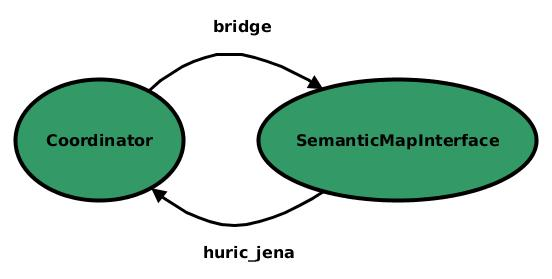
\includegraphics[width=0.8\textwidth]{imgs/topics1.jpg}
\label{fig:actions}
\caption{Data exchange between Coordinator and SemanticMapInterface}
\end{figure}


A collection of instances is retrieved and saved in a HashMap. This method performs the following SPARQL query which returns all Furniture and Drink\footnote{Furniture and Drink are classes defined in the Terminology Box} entities.

\begin{lstlisting}[language=Java]
String queryString = "PREFIX rdf: <http://www.w3.org/1999/02/22-rdf-syntax-ns#>" +
				"prefix rdfs: <"+RDFS.getURI()+">\n" +
	    		"PREFIX xsd: <http://www.w3.org/2001/XMLSchema#> " +
	    		"PREFIX hasPosition: <" + NS + POSITION +"> " +
	    		"PREFIX hasRef: <" + NS + PREF_REF +"> " +
				"prefix semantic_mapping_domain_model: <" + DOMAIN_MODEL_NS + "#> \n"+
				"prefix semantic_mapping_1: <" + SEMANTIC_MAP_NS + "#> \n"+
	    		
	    		"PREFIX coordx: <" + NS + COORD_X +"> " +
	    		"PREFIX coordy: <" + NS + COORD_Y +"> " +
	    		"PREFIX coordz: <" + NS + COORD_Z +"> " +
	    		"PREFIX prefRef: <" + NS + LEXICAL +"> " +
	    		
	    		
	    		"SELECT DISTINCT ?uri ?class ?x ?y ?z ?lex "+
	    		"WHERE {" + 
	    			"{"+
		    		"?uri a ?class ." + 
		    		"?class rdfs:subClassOf semantic_mapping_domain_model:Furniture ."+
		    		"?uri hasPosition: ?pos ." + 
		    		"?uri hasRef: ?ref ." + 
		    		"?ref prefRef: ?lex ." + 
		    		"?pos coordx: ?x . " + 
		    		"?pos coordy: ?y . " + 
		    		"?pos coordz: ?z " +  "} UNION {"+
		    		"?uri a ?class ." + 
		    		"?class rdfs:subClassOf semantic_mapping_domain_model:Drink ." +
		    		"?uri hasPosition: ?pos ." + 
		    		"?uri hasRef: ?ref ." + 
		    		"?ref prefRef: ?lex ." + 
		    		"?pos coordx: ?x . " + 
		    		"?pos coordy: ?y . " + 
		    		"?pos coordz: ?z " +  "}"+
"}" ;
\end{lstlisting}
The resulting information are embedded in a message and sent on a topic called \textit{Huric\_jena}.



\subsection{Exporting Ontology}


\subsection{Future works}

The following points assume that the robot is equipped with a spoken command recognition

Lu4r

PointCloud